In this lab, raw (uncalibrated) data was collected from five different
radiation sources:  $^{241}$Am, $^{133}$Ba, $^{60}$Co, $^{137}$Cs, and $^{152}$Eu.
The measurements were performed using a coaxial HPGe detector and a 13-bit resolution MCA,
yielding 8192-bin spectra. It is assumed that each of these measurements were
taken with each source at the same location and distance from the detector.
All raw data collected is plotted in Figure ~\ref{fig:raw}.



\begin{figure}[H]
\begin{center}
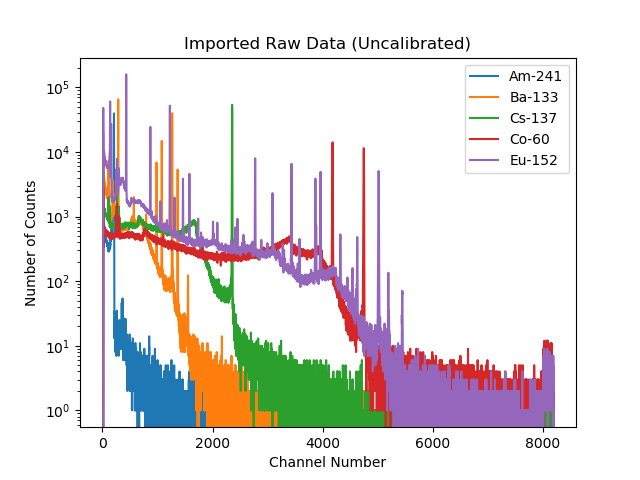
\includegraphics[width=.7\linewidth]{../images/rawdata.png}
\caption{Calibrated Americium and Cesium Spectrum
\label{fig:raw}}
\end{center}

\end{figure}


The gamma energies of interest are given in Table
\ref{tab:src}, were primarily chosen based on their
branching ratios, as those with the highest branching ratios tend to be
the most visible within a spectrum.

\begin{table}[H]
  \begin{center}
    \begin{tabular}{cccc}
      % \textbf{Source} & \textbf{Energy (keV)} & \textbf{B_ (\%)} \\
      %\hline
      \textbf{Source} & \textbf{$E_{\gamma}$ (keV)} & \textbf{Branching Ratio (\%)} \\
      $^{241}$Am    &  59.541   &    35.9(4)    \\
      $^{133}$Ba    &  80.997   &     36.68   \\
                    &  356.017   &      62.05(19) \\
      $^{60}$Co     &  1173.237  &    99.973(7)   \\
                    &  1332.501  &     99.98(6)  \\
      $^{137}$Cs    &  661.657   &      85.1(2) \\
      $^{152}$Eu    &  121.781   &     28.67(2)  \\
                    &  1408.006  &      21.07(1) \\
    \end{tabular}
    \caption{Gamma-ray lines used in the calibration}
    \label{tab:src}
  \end{center}
\end{table}

A simple linear calibration method can be employed two different energy
peaks and the channels in the raw data where these peaks are believed to
correspond to.


\begin{equation}
m=\frac{E_2-E_1}{chan_2-chan_1}
\end{equation}

where m is the slope of the linear regression line, and  $E_1$ and
$chan_1$ are a single gamma energy and corresponding channel number.

The general equation of the linear regression line is:

\begin{equation}
Energy-E_1=m(channel-chan_1)
\end{equation}
